\documentclass{article}
%\usepackage{tikz}
\usepackage[margin=1in]{geometry} % full-width
%\usepackage{graphicx}


% AMS Packages
\usepackage{amsmath}
\usepackage{amsthm}
\usepackage{amssymb}

\usepackage[T1]{fontenc}
\usepackage{tikz}

% Unicode
\usepackage[utf8]{inputenc}


\theoremstyle{definition}
\newtheorem{definition}{Definition}[section]

\newtheorem{implementation}{Implementation Caml}[section]

\usepackage{listings}
\lstset{
    language=caml,
    basicstyle=\small,
    breaklines=true
}

\title{Calcul formel}
\author{DURAND Ulysse}
\everymath{\displaystyle}
\date{}
\begin{document}

\maketitle
Le but est de faire ce qui peut s'apparenter \`a un logiciel de calcul formel en caml, il doit pouvoir \'evaluer des fonctions, les d\'eriver, et pouvoir afficher leurs expressions en \LaTeX.\\
Un objectif est aussi de pouvoir renseigner les expressions des fonctions \`a traiter en \LaTeX.
On devrait \`a la fin avoir ce r\'esultat : 
\begin{lstlisting}
let fonctiona = "\frac{x+y}{ln(x-y)}";;
let fonctionb = derive "x" fonctiona;;
print_float (evalueb [|3. ; 1.|]);;print_new_line() ;
print_string (affiche fonctionb);;print_new_line() ;
(*DOIT AFFICHER*)
-1.67935843
\frac{1}{ln(x-y)}-\frac{x+y}{(x-y)(ln(x-y))^2}
\end{lstlisting}

\section {Repr\'esentation des fonctions}
Nous traiterons d'expressions alg\'ebriques repr\'esent\'ees par des arbres d'expression.\\

l'arbre suivant repr\'esente l'expression alg\'ebrique $\frac{x+3}{-y}$ : \\

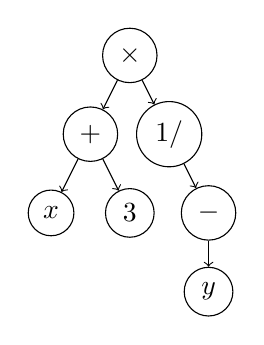
\begin{tikzpicture}[yscale=-0.5,xscale=0.5]
\node [circle, draw=black] (A) at (0,0) {$\times$};
\node [circle, draw=black] (B) at (-1,2) {+};
\node [circle, draw=black] (C) at (-2,4) {$x$};
\node [circle, draw=black] (D) at (0,4) {$3$};
\node [circle, draw=black] (E) at (1,2) {$1/$};
\node [circle, draw=black] (F) at (2,4) {$-$};
\node [circle, draw=black] (G) at (2,6) {$y$};
\draw[->] (A) to (B);
\draw[->] (B) to (C);
\draw[->] (B) to (D);
\draw[->] (A) to (E);
\draw[->] (E) to (F);
\draw[->] (F) to (G);
\end{tikzpicture}
\\
On discernera deux types de feuilles : les variables et les constantes
Et les noeuds sont de la forme (une operation, des fils)\\
d'o\`u une telle impl\'ementation en Caml :
\begin{lstlisting}
type operation = {nbvar : int ;affichage : string ; evaluation : float array->float ; derive : deriv}
and expression = 
    C of float |
    V of int |
    F of operation * (expression array)
and deriv = NonDeriv | Deriv of ((expression array)->(expression -> expression) -> expression);;
\end{lstlisting}
Les variables sont caract\'eris\'ees par un entier ($x_i, i\in\mathbb{N}$),\\ nous allons d\'etailler les caract\'eristiques affichage, evaluation et derive des op\'erations et le type deriv.\\
\subsection{affichage}
Construisons une fonction affichage : expression -> string.\\
Pour afficher une expression, nous allons expliciter pour chaque op\'eration, dans une chaine de caract\`eres, sous quelle forme l'on veut que l'affichage de la fonction se fasse. Pour cela nous utiliserons un "langage" invent\'e.
\subsubsection{le langage d'affichage d'expression}
Avec l'op\'eration plus, on veut que affichage (F(plus,[|a ; b|])) = (affichage a)\^"+"\^(affichage b).\\ Alors voici le contenu de plus.affichage : "\%|0;\%+\%|1;\%", on dit alors de retourner (affichage du fils 0) + (affichage du fils 1).\\
Notre langage doit pouvoir permettre d'avoir toutes les variables qui sont s\'epar\'ees de caract\`eres, alors pour l'op\'eration det, on veut affichage (F(det,[|x0,x1,x2|])) = "det("(affichage x0)\^","\^(affichage x1)\^","\^(affichage x2)\^")".\\ Alors voici, avec det.nbvar=3, le contenu de det.affichage : "det(\%,|a;\%)" (, le d\'elilmiteur, et a comme all pour all variables)\\
On peut imaginer une op\'erations qui doit s'afficher ainsi : ope(x3;x4;x5;...;x10) alors on aura ope.affichage = "ope\%;|3-11;\%"\\
ou encore ope(x0;x1;...;x9 / x15,x16,x17,x20,x21,...,x(n-1)) o\`u n est ope.nbvar, alors ope.affichage = "ope(\%;|-10\% / \%,|15-18;20-\%)"
\subsubsection{Compilation de ce langage}
Comment faire comprends \`a Caml ce langage ?\\
Nous allons utiliser un type d'automate particulier qui nous permettra de reconnaitre un tel langage, c'est ce qui sera appel\'e ici un automate deterministe qui \'ecrit avec m\'emoire. Il \'ecrit, c'est \`a dire qu'il reconna\^it des mots mais renvoit aussi une chaine de caract\'eres.\\
Cet automate particulier sera associ\'e \`a une fonction evaluelatex : int -> (int->char list) -> char list -> charlist\\ telle que par exemple, evaluelatex ope.nbvar funv "ope(\%;|-3\%)" = "ope("\^(funv 0)\^"(funv 1)"\^(funv 2)\^")" (nous confondrons ici string et charlist par souci de simplicit\'ee.)\\
Les d\'etails de l'automate et de sa fonction, evaluelatex, associ\'ee, seront explicit\'es dans la section 2.

\section{De quoi faire la fonction evaluelatex}
\subsection{Automates utiles}
En caml, voilà une manière d'implémenter les automates : 
\begin{lstlisting}
type ('q, 'sig) automate = ('q -> bool)*('q -> bool)*(q'*sig'*('q list));;
(*('q,'ssig) automate = (i,f,delta) correspond a un automate ('q,'sig,i,f,delta)*)
\end{lstlisting}

\subsubsection{Automate déterministe qui écrit}
\begin{definition}[Automate déterministe qui écrit]
Ce type d'automate permet de transformer un mot en un autre.\\
\begin{gather*}
    \mathcal{A} = (Q,\Sigma_1 ,\Sigma_2, i, F, \delta, \eta) \\
    i\in Q,F \in \mathcal{P} (Q)
\end{gather*}
\begin{align*} 
    \delta : Q\times \Sigma_1 &\rightarrow Q \\
    \eta : Q\times \Sigma_1 &\rightarrow (\Sigma_2 )^\star\\
    \\             
    \delta^\star : Q\times \Sigma_1 ^\star &\rightarrow Q \\
    (q,\epsilon) &\mapsto q\\
    (q,l.m) &\mapsto \delta^\star(\delta(q,l),m)\text{, avec }l\in \Sigma_1\\
    \\
    \eta^\star : Q\times \Sigma_1 ^\star &\rightarrow (\Sigma_2)^\star \\
    (q,\epsilon) &\mapsto \epsilon '\\
    (q,l.m) &\mapsto \eta(q,l).\eta^\star(\delta(q,l),m)\text{, avec }l\in \Sigma_1\\
\end{align*}

\end{definition}
Implementation en Caml : 
\begin{lstlisting}
type ('q, 'sig1, 'sig2) automatequiecrit = ('q*('sig2 list), 'sig1 ) automate;;
\end{lstlisting}
\textbf{('q,'sig1,'sig2) automatequiecrit = (i,f,g)} correspond \`a un automate $('q,'sig1,'sig2,i,f,delta,eta)$. Supposons $g$ sous la forme $g((q,m),l) = (q',p::m)$, alors $delta(q,l) = q'$ et $eta(q,l) = p$
\newpage
\subsubsection{Automate qui écrit avec une mémoire}

\begin{definition}[Automate qui écrit avec mémoire]
Ce type d'automate n'a pas de d'intérêt théorique vu que la mémoire est finie, mais a un intérêt pratique.

\begin{gather*}
    \mathcal{A} = (Q,\Sigma_1,\Sigma_2, S_m, i, F, \delta, \eta) \\
    Q,\Sigma_1,\Sigma_2,i,F \text{ restent inchangés}
\end{gather*}
\begin{align*}
    \delta : Q\times S_m \times \Sigma_1 &\rightarrow Q \times S_m \\
    \eta : Q\times S_m \times \Sigma_1&\rightarrow (\Sigma_2 )^\star\\
    \\             
    \delta^\star : Q\times S_m \times \Sigma_1^\star &\rightarrow Q \\
    (q,M,\epsilon) &\mapsto q\\
    (q,M,l.m) &\mapsto \delta^\star(\delta(q,M,l),m)\text{, avec }l\in \Sigma\\
    \eta^\star : Q\times S_m\times \Sigma_1^\star &\rightarrow (\Sigma_2)^\star \\
    (q,M,\epsilon) &\mapsto \epsilon '\\
    (q,M,l.m) &\mapsto \eta(q,M,l).\eta^\star(\delta(q,M,l),m) \text{, avec }l \in \Sigma_1\\
\end{align*}
\end{definition}
Il s'agit en fait d'un automate qui écrit avec $Q' = Q \times S_m$\\
Implementation en Ocaml : \\
\begin{lstlisting}    
type ('q, 'sm, 'sig1, 'sig2) automatequiecritavecmemoire = ('q*'sm,'sig1,'sig2) automatequiecrit
\end{lstlisting}
\textbf{('q,'sm,'sig1,sig2) automatequiecritavecmemoire : (i,f,g)} correspond \`a un automate
qui ecrit avec m\'emoire $('q,sig1,sig2,sm,i,f,delta,eta)$.
Supposons $g$ sous la forme $g((q,m,mem),l) = ((q',mem'),p@m)$,
alors $delta((q,mem),l) = (q',mem')$ et $eta((q',mem'),l) = p$\\\\
Pour les représenter graphiquement, nous ferons comme les automates, mais avec des annotation sur les arêtes différentes :\\
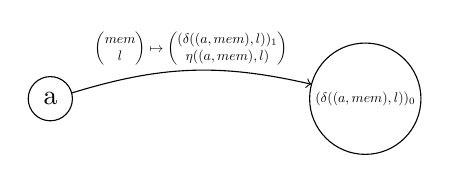
\begin{tikzpicture}
	\node[shape=circle,draw=black] (0) at (0,0) {a};
	\node[shape=circle,draw=black,scale = 0.5] (1) at (4,0) {$(\delta((a,mem),l))_0$};
	\draw [->,bend left=15] (0) to node[above, scale=0.5] {$\begin{pmatrix} mem \\ l \end{pmatrix} \mapsto \begin{pmatrix} (\delta((a,mem),l))_1 \\ \eta((a,mem),l) \end{pmatrix} $} (1);
\end{tikzpicture}
\subsection{Et dans notre cas}
Notre automate qui écrit avec une mémoire pour \'ecrire du latex :\\ 
avec $n$ un entier et $N = \{"0","1","2","3","4","5","6","7","8","9"\}$\\
\resizebox{\textwidth}{!}{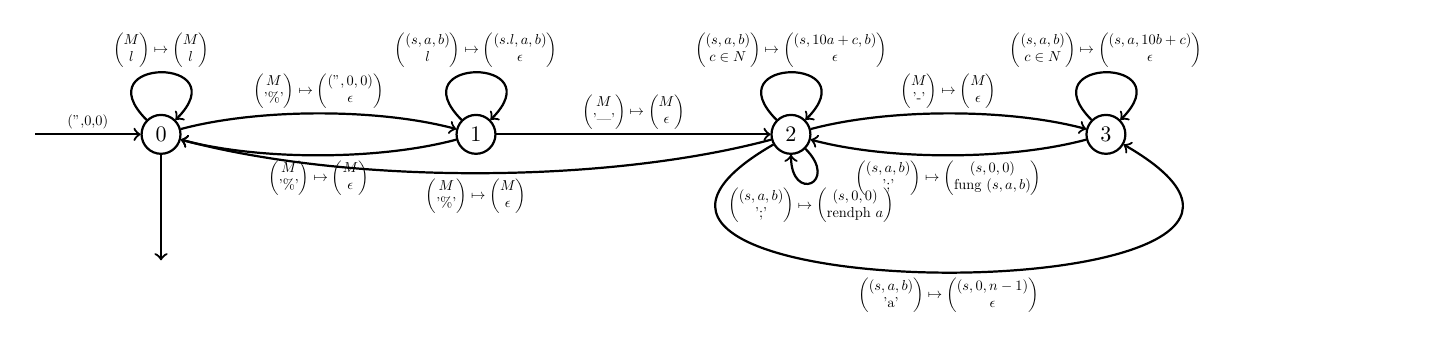
\begin{tikzpicture}[thick,scale=0.8, every node/.style={transform shape}]
	\def\sc{0.65};
	\node [shape=circle,draw=black] (0) at (0, 0) {0};
	\node [shape=circle,draw=black] (1) at (5, 0) {1};
	\node [shape=circle,draw=black] (2) at (10, 0) {2};
	\node [shape=circle,draw=black] (3) at (15, 0) {3};
	\node [] (4) at (-2, 0) {};
	\node [] (5) at (0, -2) {};
	\draw [->, in=165, out=15, looseness=0.75] (0) to node [ above, scale=\sc] {$\begin{pmatrix} M \\ \text{'\%'} \end{pmatrix} \mapsto \begin{pmatrix} (\text{''},0,0) \\ \epsilon \end{pmatrix} $} (1);
	\draw [->, bend left=15, looseness=0.75] (1) to node [ below, scale=\sc] {$\begin{pmatrix} M \\ \text{'\%'} \end{pmatrix} \mapsto \begin{pmatrix} M \\ \epsilon \end{pmatrix} $} (0);
	\draw [->, bend left=15, looseness=0.75] (2) to node [ below, scale=\sc] {$\begin{pmatrix} M \\ \text{'\%'} \end{pmatrix} \mapsto \begin{pmatrix} M \\ \epsilon \end{pmatrix} $} (0);
	\draw [->, in=45, out=135, loop] (1) to node [ above, scale=\sc] {$\begin{pmatrix} (s,a,b) \\ l \end{pmatrix} \mapsto \begin{pmatrix} (s.l,a,b) \\ \epsilon \end{pmatrix} $} ();
	\draw [->] (1) to node [ above, scale=\sc] {$\begin{pmatrix} M \\ \text{'|'} \end{pmatrix} \mapsto \begin{pmatrix} M \\ \epsilon \end{pmatrix} $} (2);
	\draw [->, in=45, out=135, loop] (2) to node [ above, scale=\sc] {$\begin{pmatrix} (s,a,b) \\ c \in N \end{pmatrix} \mapsto \begin{pmatrix} (s,10a+c,b) \\ \epsilon \end{pmatrix} $} ();
	\draw [->, bend left=15, looseness=0.75] (2) to node [ above, scale=\sc] {$\begin{pmatrix} M \\ \text{'-'} \end{pmatrix} \mapsto \begin{pmatrix} M \\ \epsilon \end{pmatrix} $} (3);
	\draw [->, in=45, out=135, loop] (3) to node [ above, scale=\sc] {$\begin{pmatrix} (s,a,b) \\ c \in N \end{pmatrix} \mapsto \begin{pmatrix} (s,a,10b+c) \\ \epsilon \end{pmatrix} $} ();
	\draw [->, in=45, out=135, loop] (0) to node [ above, scale=\sc] {$\begin{pmatrix} M \\ l \end{pmatrix} \mapsto \begin{pmatrix} M \\ l \end{pmatrix} $} ();
	\draw [->, bend left=15, looseness=0.75] (3) to node [ below, scale=\sc] {$\begin{pmatrix} (s,a,b) \\ \text{';'} \end{pmatrix} \mapsto \begin{pmatrix} (s,0,0) \\ \text{fung } (s,a,b) \end{pmatrix} $} (2);
	\draw [->, bend right=150, looseness=2.50] (2) to node [ below, scale=\sc] {$\begin{pmatrix} (s,a,b) \\ \text{'a'} \end{pmatrix} \mapsto \begin{pmatrix} (s,0,n-1) \\ \epsilon \end{pmatrix} $} (3);
	\draw [->, in=-90, out=-45, loop] (2) to node [below, scale=\sc] {$\begin{pmatrix} (s,a,b) \\ \text{';'} \end{pmatrix} \mapsto \begin{pmatrix} (s,0,0) \\ \text{rendph } a \end{pmatrix} $} ();
	\draw [->] (4.center) to node[above,scale=\sc] {(\text{''},0,0)} (0);
	\draw [->] (0) to (5.center);
\end{tikzpicture}
} \\\\
Si A est cet automate qui écrit, $n = 6$, funv$(s,a,b) = "x\_a"$,\\ fung $(s,0,3)$ = (funv  $0$).s.(funv $1$).s.(funv $2$).s.(funv $3$),\\\\
$\eta^\star (0,(\text{''},0,0),$ 
\verb|\frac{{%|\textbar\verb|0;%+%|\textbar\verb|15;%}^{(%*|\textbar\verb|1-4;%)}}| ) =\\
\verb|\frac{{x_0+x_15}^{x_1*x_2*x_3}}{x_0+x_1+x_2+x_3+x_4+x_5}|

\end{document}

